\documentclass[12pt, letterpaper]{article}
\usepackage{macros}
\usepackage{bbm}
\usepackage{longtable}
\usepackage{titlesec}
\singlespacing



\titleformat{\section}
  {\normalfont\sffamily\Large\bfseries}
  {\thesection}{1em}{}
\titleformat{\subsection}
  {\normalfont\sffamily\large\bfseries}
  {\thesubsection}{1em}{}
  
\titleformat{\subsubsection}
  {\normalfont\sffamily\normalsize\bfseries}
  {\thesubsubsection}{1em}{}
  
\hypersetup{urlcolor=Purple}

% \singlespacing
\newgeometry{margin=1in}
\title{\sffamily\bfseries{Prediction of the 2018 Midterm Elections Final Project II}}
\author{Jiafeng Chen\thanks{Harvard College, \url{jiafengchen@college.harvard.edu}} \and Joon Hyuk Yang\thanks{Harvard College, \url{joonhyukyang@college.harvard.edu}}}
\begin{document}
\maketitle

\section{Areas for Improvement}
\label{sec:model}

\subsection{Data and Preprocessing}
As discussed in Part I, we used a dozen features to inform our prior $Y \sim \mathcal{N}(\mu_0, \Sigma_0)$, and subsequently updated the posterior, once with the generic ballot poll and the second time via district-wide poll. There was room for improvement in collecting data for the prior as well as the posterior update, respectively.

One primary point of concern that was evident was the reliability of data. As the class collectively contributed features from various sources, some were less reliant than others. For instance, the gender of the candidiate, upon manual inspection, was wrong in many cases. We used the gender-guesser library to account for this while marking gender neutral names as 0.5. This means that (1) we could have improved our data cleaning process by looking up each candidate and filling in inconclusive entries, and (2) features such as presidential approval or education level may have suffered from inaccurate data reporting or exhibit high variance by being a point estimate as opposed to an aggregate over surveys from longer periods of time.

In Part I, we also discussed the effectiveness of Google Trends's relative popularity of search queries. However, there were several assumptions made that may have introduced bias in our results. First, search frequency is a good proxy for interest, but it does not translate to support. We can imagine various scenarios such as an incumbent candidate not having as many search queries by virtue of already being well-known, or having a much higher search query due to a negative press release. As our model relies on a linear model with at most a second degree basis transform, tracing complex, non-linear relationships was limited when simiply fitting with regularized regression. Second, for certain states (especially those with a low population), acquiring search frequency ratio of candidate names at a State-level granularity was impossible because a lack of absolute number of queries. We imputed these ratios with the ratios of a nation-wide search, which is itself a biased assumption, since these states were primarily red states while the aggregate nation-wide search is primarily dominated by more liberal states. A final point to make is that even for states where there are enough queries to return a state-level ratio, such as in Alaska (\Cref{fig:candidate_only}), the resulting ratio alone may not be a discerrning indicator for candidate preference.

\begin{figure}[tbh]
  \centering
  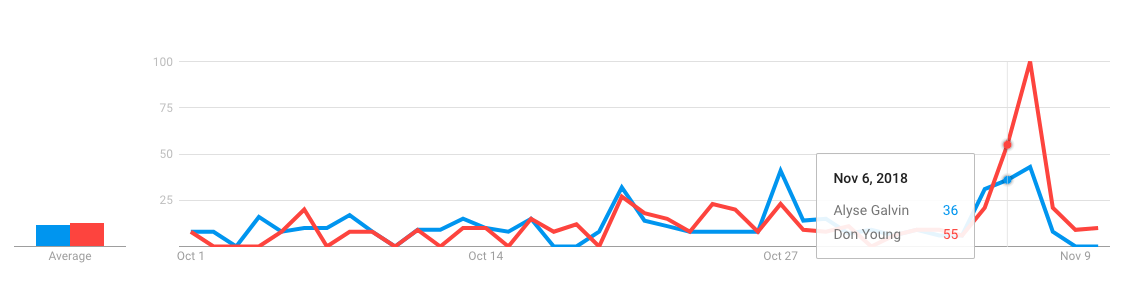
\includegraphics[scale=0.4]{alaska_candidate}
  \caption{Google Trends search frequency ratio of Democratic vs. Republican candidate in Alaska at large.}
  \label{fig:candidate_only}
\end{figure}

A better estimate can be had by examining key issues that each candidate or party is putting at the forefront of the campaign and to do a state-by-state trends ratio search to identify which issues are important to voters. For instance, \Cref{fig:trends_issues} shows the Google Trends frequency results for four key issues: guns, defense, healthcare, and wellness. The first two are the flagship areas in which Alaska's Republican candidate emphasized, while the latter two are those prioritized by the Democratic candidate. The overall running average of these issues in Alaska suggests that there is ample room to augment our data by feeding in a more holistic picture of search query frequency ratios on topics that are brought forth by candidates. Don Young, the Republican, took Alaska's seat at the House.

\begin{figure}[tbh]
  \centering
  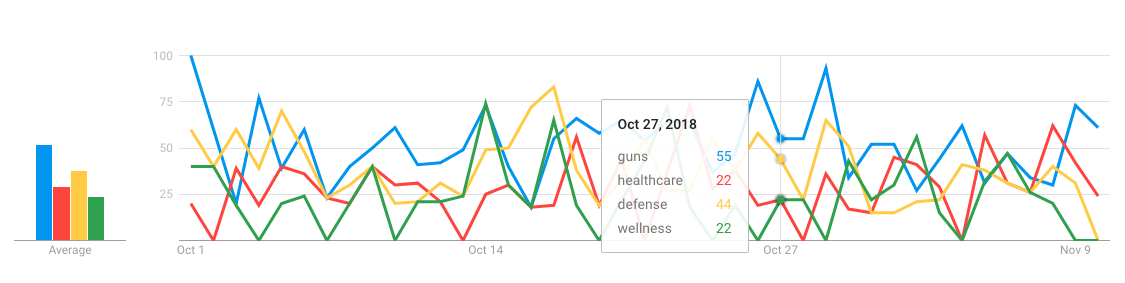
\includegraphics[scale=0.4]{trends_issues}
  \caption{Google Trends search frequency ratio in Alaska on guns, healthcare, defense, and wellness. On average, guns are more frequently queried compared to healthcare, and defense more frequently than wellness.}
  \label{fig:trends_issues}
\end{figure}

Furthermore, access to anonymized browsing history from Interet Service Providers (ISPs) may allow us to uncover latent sentiments that may be interpolated at poll-time. This will be further expounded in Model Selection. 

\section{Models}
\subsection{Browsing History in Model Update}
Our prediction results rely heavily on the validity of our posterior update, which is dominated by how informative the polling data may be. However, polling data may be noisy at best and worse misleading. In fact, each pollster has such high variance that there are pollster ratings, which Part I did not explicitly take into account. The aggregate or \textit{overall} trend in polls is what Nate Silver explains as being of greater interest.\footnote{Silver argues that both macro and micro trends from polling data are important--the former being the aggregate poll result and the latter being the pollster ratings. More information at fivethirtyeight.com/features/which-pollsters-to-trust-in-2018} In order to mitigate the noisy nature of polls and the effects of poll-to-poll variance, given more resources, we could introduce an intermediate step between poll data and votes by introducing browsing data.

On a high level, we use browsing history $B$ for each district and assume that given this, polling results are distributed Normally. Instead of solely relying on voting results to fit the parameters of $Z$, we now introduce a tertiary variable through which we can (1) potentially use to directly compute $Y \ | \ B$ or in our case, more parochially, (2) easily derive the $\Sigma_Z$ by calculating $\hat{Z} \ | \ B$ and calculating the variance of the newly acquired live poll against our $\hat{Z}$.

\begin{figure}[tbh]
  \centering
  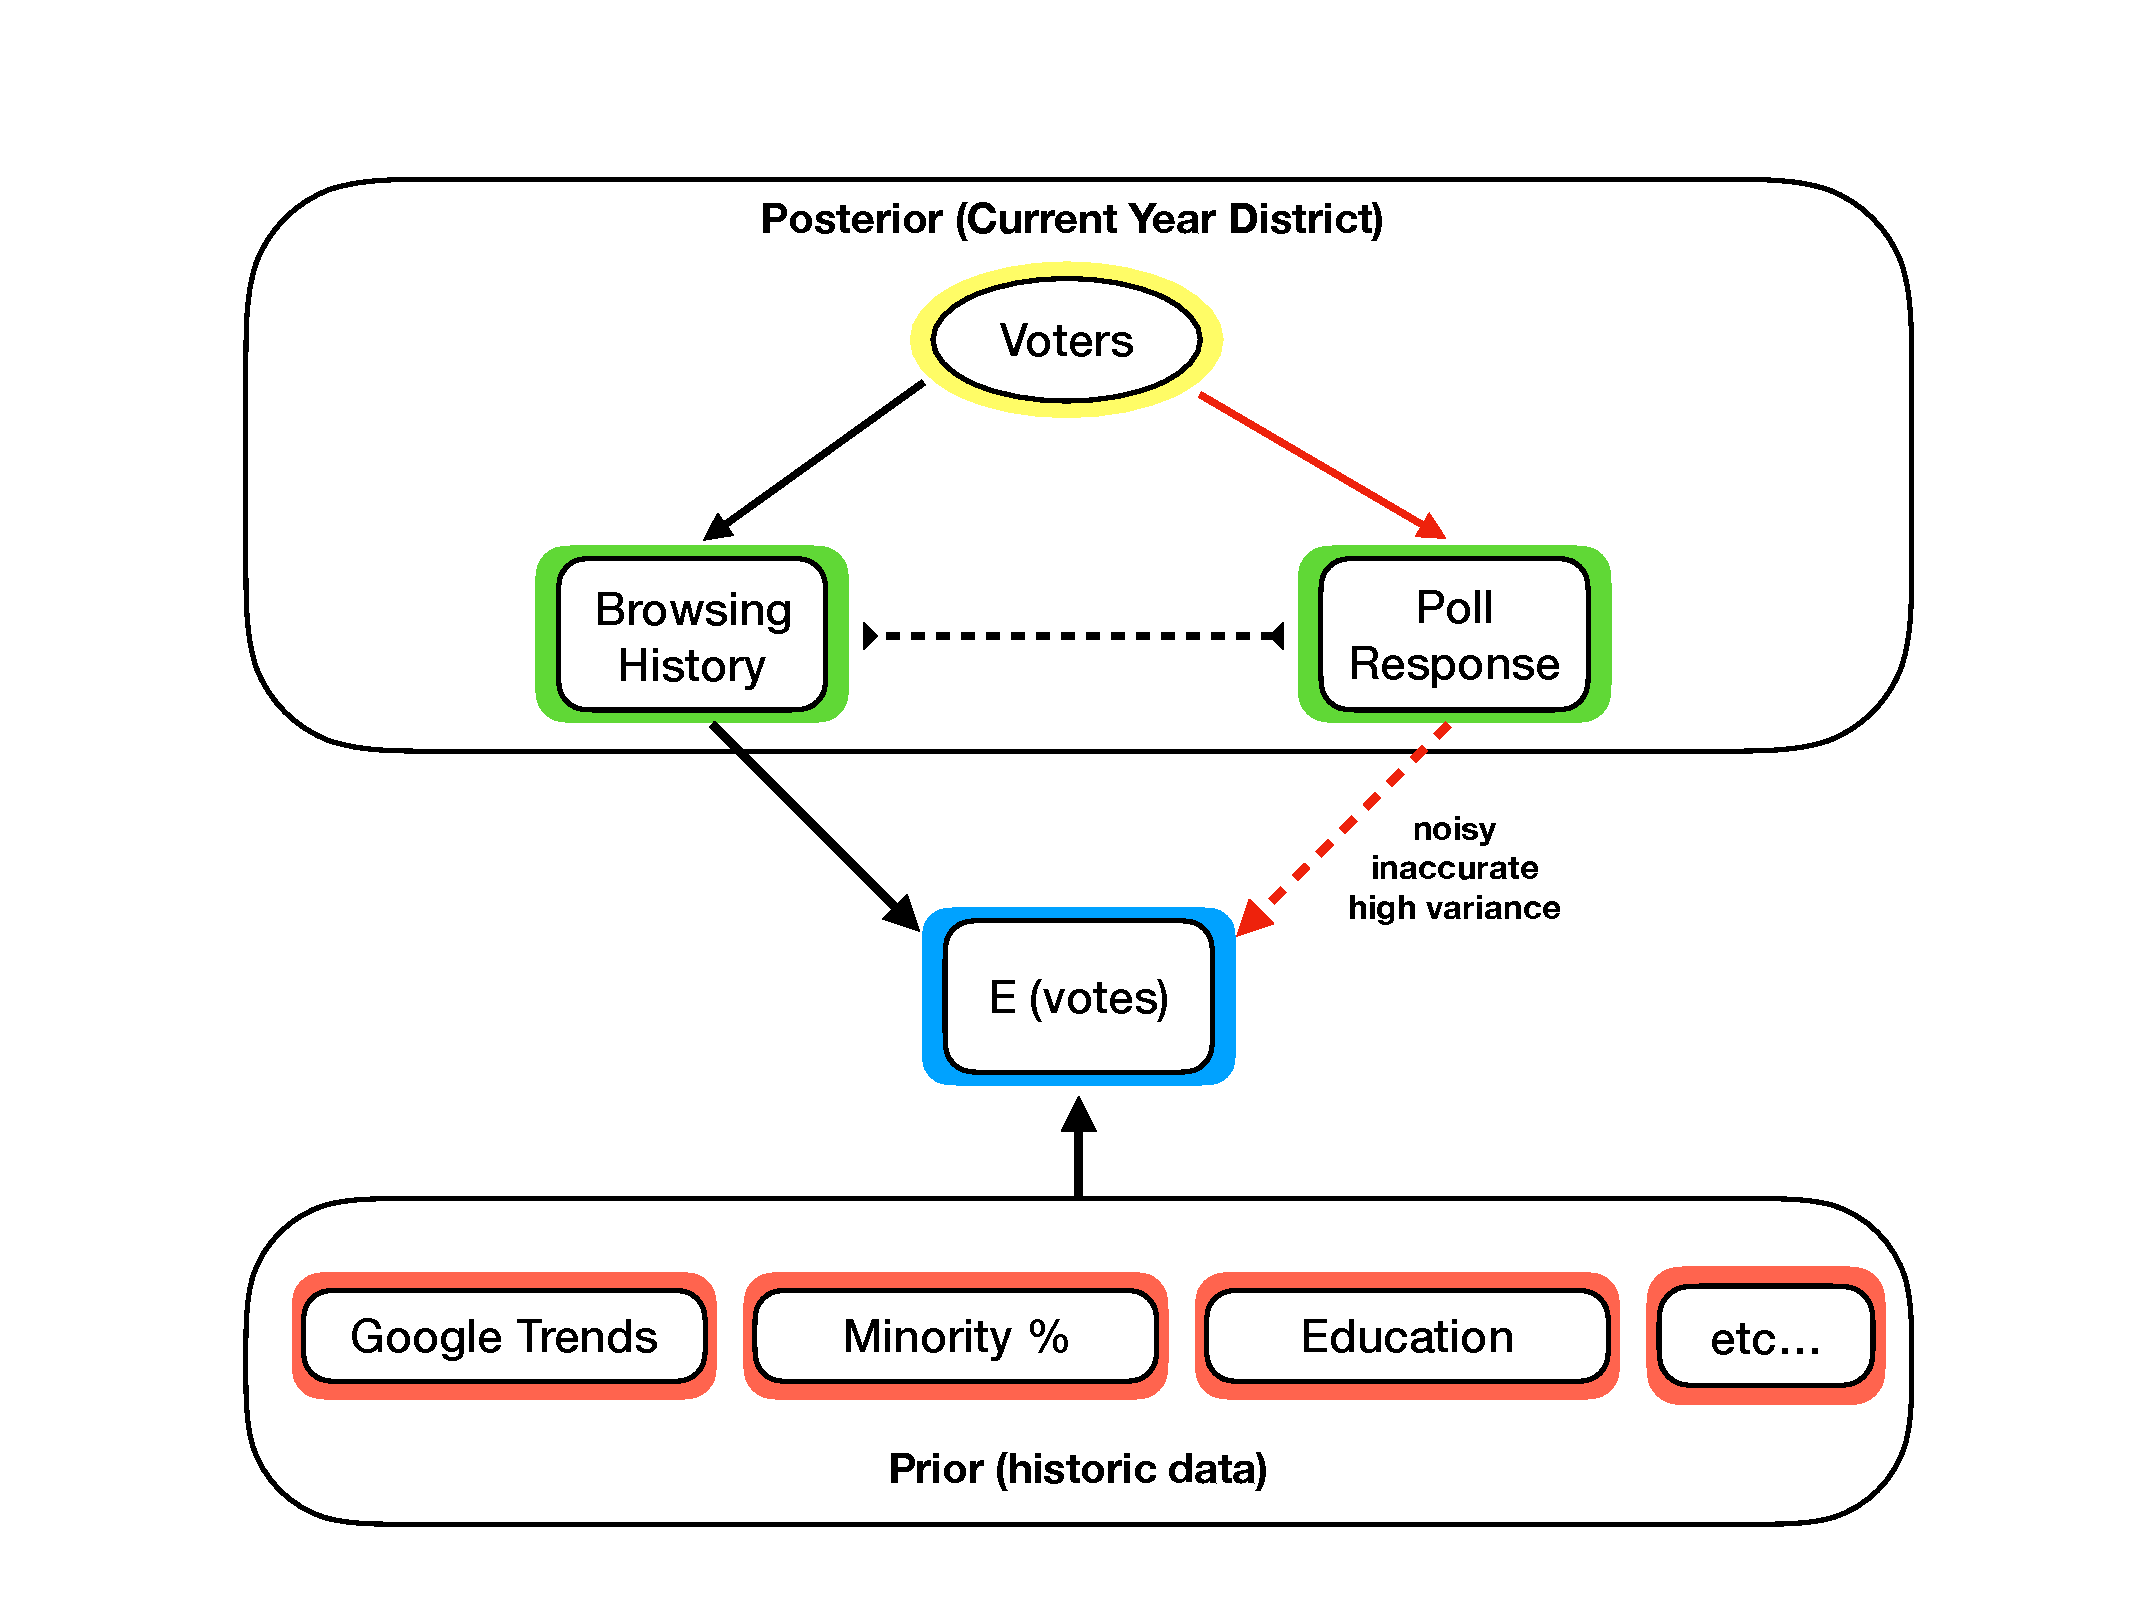
\includegraphics[scale=0.4]{browsing_diagram.pdf}
  \caption{Diagrammatic view of incorporating browsing history as an alternative to poll-based posterior update.}
  \label{fig:browsing}
\end{figure}

The method entails the use of historic polling data and browsing history to fit a function in each district that captures the relationship (\Cref{fig:browsing}). Given ISP's data on how a registered Democrat or Republican browses during the same time a poll is conducted, we can fit parameters of a function as simple as a regularized regression or even a neural network. This model selection would depend on how we record browsing history; if we filter down to a few key websites and monitor voters' respective traffic, a simple regression model may be sufficient, while if we chose to incorporate a large number of features, we may choose a neural network of the form
\begin{align*}
H_m &= \sigma(\alpha_{0m} + \alpha_m^TB), \text{\ where \ } m \in [1,M]\\
Z_{k}^{(j)} &= \beta_{0k}^{(j)} + \beta_k^{(j)T}H, \text{\ where \ } k \in \{0, 1\}\\
\end{align*}
where the activation function that introduces non-linearity $\sigma(\cdot)$ could be a sigmoid, a Rectified Linear Unit (ReLU), or Gaussian radial basis function; $H$ is the hidden layer(s) with $M$ units; and $Z_k^{(j)}$ is the aggregate polling result of district $j$ for party $k$ in the timeframe during which browsing history $B$ is collected. Using stochastic gradient descent as our fitting method, we can fit the parameters to translate 

The biggest drawback of this model is the availability of historic browsing and polling data.


\bibliographystyle{jpe}
\bibliography{main.bib}
\newpage
\appendix

\section{District-by-district projections}
\label{sec:district_results}


\section{Figures}
\label{sec:figures}


\end{document}
